Physically, a quartz crystal microbalance manifests itself as a thin disc
of crystalline quartz, \ce{SiO2}, with metal electrodes deposited on either
side (\Figure{fig:qcmholding}).  The crystalline structure is specifically
$\alpha$-quartz, organized in a trigonal system which is pizeoelectric.
Typically the crystal employs the ``AT-cut'' -- a cut at an angle of
\SI{35.25}{\degree} with respect to the crystallographic axis.  In the
AT-cut, the vibrational state is dominated by the thickness shear mode,
setting up transverse shear waves along the faces of the crystal
(\Figure{fig:qcmshearwave}.  The AT-cut quartz also has the convienence of
a zero frequency temperature coefficent at \SI{25}{\celsius}.

When an object is deposited on the crystal surface, the surface acoustic
waves will interact with a sample and the resonance frequency of the hybrid
system will change.  This is the principle of QCM sensing.
\begin{figure}[ht]
 \centering
 	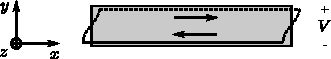
\includegraphics[keepaspectratio]{qcm/figures/qcm_shearmode.pdf}
	\caption{Conceptual drawing of a transverse shear wave.}
 \label{fig:qcmshearwave}
\end{figure}
